\documentclass[letter, 10pt]{article}
% Change "article" to "report" to get rid of page number on title page
\usepackage{amsmath,amsfonts,amsthm,amssymb}
\usepackage{setspace}
\usepackage{graphicx,float,wrapfig}
%\usepackage{parskip}
\usepackage{enumerate}

\usepackage{tikz}
\tikzset{auto}

\usepackage{fourier}
\usepackage[T1]{fontenc}
\usepackage[protrusion=true,expansion=true]{microtype}

% In case you need to adjust margins:
\topmargin=-0.45in      %
\evensidemargin=0in     %
\oddsidemargin=0in      %
\textwidth=6.5in        %
\textheight=9.0in       %
\headsep=0.25in         %
\parindent=0in

\usepackage[nodayofweek]{datetime} \usdate
% Pdf metadata
\pdfinfo{  /Author (Blake Riley)
           /Title (Econ 533 Handout 5)
           /Keywords ()
           /ModDate (D:\pdfdate)}

\newtheoremstyle{basic}% name
   {5pt}% Space above
   {5pt}% Space below
   {\itshape \leftskip=1em}% Body font
   {-1em}% Indent amount
   {\bfseries}% Theorem head font
   {:}% Punctuation after theorem head
   { }% Space after theorem head
   {}% Theorem head spec (can be left empty, meaning `normal')
\theoremstyle{basic}
\newtheorem{exercise}{Exercise}[section]
\newtheorem{definition}{Definition}[section]
\newtheorem{theorem}{Theorem}[section]
\newtheorem{lemma}[theorem]{Lemma}


%%%%%%%%%%%%%%%%%%%%%%%%%%%%%%%%%%%%%%%%%%%%%%%%%%%%%%%%%%%%

% Custom commands

\newcommand{\R}{\mathbb{R}}
\newcommand{\N}{\mathbb{N}}
\newcommand{\E}{\operatorname{E}}
\renewcommand{\P}{\operatorname{Pr}}
\newcommand{\Var}{\operatorname{Var}}
\newcommand{\Cov}{\operatorname{Cov}}
\newcommand{\cond}{\,|\,}
\newcommand{\bigcond}{\;\big|\;}
\newcommand{\argmax}{\mathop{\operatorname{arg\,max}}}
\newcommand{\noti}{{{\scriptscriptstyle-}\!i}}
\newcommand{\notj}{{{\scriptscriptstyle-}\!j}}
\newcommand{\notij}{{{\scriptscriptstyle-}\!\{i,j\}}}
\newcommand{\I}{\mathbb{I}}
\newcommand{\tto}{\twoheadrightarrow}

%%%%%%%%%%%%%%%%%%%%%%%%%%%%%%%%%%%%%%%%%%%%%%%%%%%%%%%%%%%%%
%%%%%%%%%% The main document content
%%%%%%%%%%%%%%%%%%%%%%%%%%%%%%%%%%%%%%%%%%%%%%%%%%%%%%%%%%%%%

\begin{document}
\begin{spacing}{1.0}

\noindent
\textbf{Handout 5} \\
Econ 533 \\
March 13, 2015 \\
TA: Blake Riley \\

\section{Mechanism Design with Money}
\label{sec:vick-clarke-grov}

The Gibbard-Satterthwaite theorem applies to mechanisms that work on all possible
preferences. By restricting the setting, we can recover positive results. One
particularly fruitful setting is when agents have quasi-linear preferences over
transfers. The ability of the mechanism designer to charge or compensate agents opens
up new possibilities for incentives besides changing the direct outcome. With new
possibilities comes new problems, though. The designer must to be careful agents
aren't charged so much they're no longer interested in participating. The mechanism
might also run a surplus or deficit if transfers between agents don't balance out.

\begin{definition}
  Agent $i$ has \textbf{quasi-linear preferences} over transfers iff the
  agent's utility function is representable as $u_i(\theta_i, a, t_i) =
  v_i(\theta_i,a)+t_i$ for some function $v_i(\theta_i,a)$.
\end{definition}

For now, we are concerned with implementing an efficient choice. Later we
will consider alternative objectives like maximizing the revenue of the
designer.

\begin{definition}
  A choice $a^* \in A$ is \textbf{efficient} in state $\theta$ iff $a^* \in
  \operatorname{argmax}_{a\in A} \sum_i v_i(\theta_i, a)$.
\end{definition}

\begin{definition}
  The \textbf{efficiency correspondence} $\bar{F}:\Theta \tto A$ assigns to
  each state the efficient choices. Similarly, an \textbf{efficiency
    decision rule} is a function that assigns some efficient choice.
\end{definition}

\begin{definition}
  In a setting with transfers and $n$ agents, a social choice function
  $f:\Theta \to A\times \R^n$ is a pair $(d(\theta), t(\theta))$, where $d$
  is a decision rule which selects some collective option from $A$ and $t$
  defines a vector of transfers to agents (with negative transfers being
  payments by agents).
\end{definition}

We'll typically assume the designer can't run a deficit, so the feasible
mechanisms are self-financing ones.

\begin{definition}
  A transfer function $t$ is \textbf{feasible} if $\sum_i t_i(\theta) \leq
  0$ for all $\theta \in \Theta$. A transfer function is \textbf{ex-post
    budget balanced} if $\sum_i t_i(\theta) = 0$ for all $\theta$.
\end{definition}

We don't want to assume agents are forced to participate, so we have the
notion of ex-post individual rationality.

\begin{definition}
  A social choice function $(d,t)$ is \textbf{ex-post
    individually rational} iff $v_i(\theta_i,F(\theta))+
  t_i(\theta) \geq 0$ for all $i$ and $\theta_i$.
\end{definition}

The \textit{ex-post} label refers to these properties holding for all
possible realizations of types. Alternately, we can consider
\textit{ex-ante} or \textit{ex-interim} properties that hold in expectation
over all type profiles or in expectation conditional on one agent's type,
respectively. More on these in later classes.

\section{Vickrey-Clarke-Groves Mechanisms}
\label{sec:vickr-clarke-grov}

The basic VCG mechanism is a rule for selecting the efficient choice along
with specific monetary transfers. Here ``basic'' refers to the fact that an
entire class of mechanisms have the same properties.

\begin{definition}
  Given an efficient decision rule $d$ and reports $\theta^*$ of the $n$
  agents, the \textbf{basic VCG} mechanism selects $d(\theta^*)\in A$ and
  allocates transfers \[t_i^{VCG}(\theta^*)=\sum_{j\neq i}
  v_j(\theta_j^*,d(\theta^*))\]
\end{definition}

\begin{definition}
  Given an efficient decision rule $d$, a mechanism is in the \textbf{VCG
    family} or is a \textbf{Groves mechanism} if for reports $\theta^*$ of
  the $n$ agents
  \begin{enumerate}
  \item The mechanism selects $d(\theta^*) \in A$.
  \item The transfer has the form $t_i(\theta^*) = t_i^{VCG}(\theta^*)
    + h_i(\theta_{-i})$, for any set of $n$
    functions $h_i:\Theta_{-i} \to \R$.
  \end{enumerate}
\end{definition}

This additional term $h_i(\theta_{-i})$ is sometimes called an
individualized tax. On an exam, if you are asked to define the family of
VCG mechanisms for a given problem, you have to adjust this definition and
find the objective and transfers up to some arbitrary functions.

\hspace{1em} Notice that with a VCG mechanism, each agent has the social welfare
criterion as his own objective, plus something that is unchanged by his
report. The individuals' incentives are now aligned with the group, so
honest reporting becomes (weakly) dominant. Surprisingly, the converse is
also true.
\begin{theorem}
  (Groves 1973) The family of VCG mechanisms is dominant strategy incentive
  compatible (strategy-proof).
\end{theorem}
\begin{theorem}
  (Green and Laffont 1977) Conversely, if $d$ is an efficient decision
  rule, the social choice function $(d,t)$ is strategy-proof, and the type
  spaces are complete in the sense that each $a \in A$ is selected by $d$
  for some type profile, then the mechanism is in the VCG family.
\end{theorem}
Even weakening dominant-strategy IC to Bayesian IC (which we'll investigate
later) doesn't change the class of efficient mechanisms:
\begin{theorem}
  (Williams 1999) Every efficient and Bayesian incentive-compatible
  mechanism with transfers gives the same interim payoffs as some Groves
  mechanism, assuming type spaces are connected, open subsets of Euclidean
  space and interim valuations are continuously differentiable.
\end{theorem}

We still have an open question about the ``best'' $h_i$'s. If we let $h_i$
be zero as in the basic mechanism, then each player receives large
transfers, violating feasibility. Intuitively, we would prefer something
like a Pigouvian tax, where transfers reflect the externality of adding a
person to society.

\begin{definition}
  The \textbf{Clarke pivotal mechanism} for an efficient decision rule $d$
  is a VCG mechanism where \[t_i(\theta) = \sum_{j \neq i} v_j(\theta_j,
  d(\theta)) - \max_{a\in A} \sum_{j\neq i} v_j(\theta_j, a)\]
\end{definition}

\begin{theorem}
  If $v_i(\theta_i,a)\geq 0$ for all $i$, the pivotal mechanism always
  makes negative transfers, is feasible, and is ex-post individually
  rational.
\end{theorem}

Sometimes the pivotal mechanism is referred to as \emph{the} VCG mechanism,
while any other choice of $h_i$'s is \emph{a} VCG mechanism or a Groves
mechanism.

\section{Virtues and Vices of the VCG}
\label{sec:virtues-vcg}

The work leading up to the VCG was a theoretical
\emph{tour-de-force}. The characterization of how to achieve
perfect efficiency in dominant strategies is elegant and
appealing. However, while shedding insight into the workings of mechanisms,
it's not necessarily something you'd want to use. ``Thirteen reasons why the
VCG process is not practical'' (Rothkopf 2007) documents these clearly:
\begin{enumerate}
\item the nonexistence of dominant-strategy equilibria in models with reasonable bid preparation costs;
\item problems associated with the disclosure of valuable confidential
  information;
\item the exponential growth of effort related to bid preparation and bid
  communication;
\item the NP-completeness of the winner determination problem;
\item the dominant strategy equilibrium is a weak equilibrium and there may
  exist alternative weak equilibria;
\item problems related to capital-limited bidders;
\item problems associated with various kinds of cheating
  including:
  \begin{enumerate}
  \item false bids by the bid taker,
  \item conspiracies by competing bidders,
  \item conspiracies in two-sided markets between bidders offering
    to sell and those offering to buy,
  \item  and the use of false-name bids by single bidders;
  \end{enumerate}
\item the fact that strategies in sequences of strategy-proof auctions may
  not be strategy-proof;
\item the fact that the process can be revenue deficient.
\end{enumerate}
The first three problems are common to most direct mechanisms in
combinatorial settings. Direct mechanisms are very useful theoretically,
but communication costs (from transmission, preparation, or
privacy-violations) break the revelation principle.

\hspace{1em}
Notice that the efficiency of the VCG applies only to the
allocation/decision, assuming negative transfers aren't lost from the
economy. The pivotal mechanism actually turns out to maximize total
payments among feasible, ex-post IR mechanisms, which can be a good thing when
payments are seen as revenue. However, if there isn't someone external to
absorb the payments, the benefit of efficiency in decisions is partially
reduced. 

\hspace{1em}
Every cloud has a silver lining though. Each deficiency with the VCG is a
new opportunity for budding market designers. For instance, redistribution
mechanisms \footnote{See Ruggerio (2006), ``Optimal decision-making with
  minimal waste'', Guo and Conitzer (2010), ``Optimal-in-expectation
  redistribution mechanisms'', and Ruggerio (2012) ``Fairness and welfare
  through redistribution when utility is transferable'', among others.}
return some of the pivotal mechanism transfers back to participants while
maintaining feasibility. In particular, given pivotal mechanism payments,
Ruggerio's redistribution mechanism reduces each positive payment by the
total revenue that would have been collected if the agent reported his
minimal possible valuation and splits it equally between all agents
(including himself).  Clippel et al. (2012), ``Destroy to save'' shows that
allowing a tiny bit of inefficiency in the allocation can substantially
reduce the amount of surplus taken from participants, improving overall
participant welfare.

\newpage
\section{Exercises}
\label{sec:exercises}

\begin{exercise}
  Describe the VCG family, pivotal mechanism, and redistribution mechanism
  outcomes for the following applications:
  \begin{enumerate}
  \item Living arrangements: Three grad students, Abel, Baker, and Charlie,
    are renting a three-bedroom apartment together. The rent is \$600 and
    they've committed to paying equal shares. Now they have to decide who
    gets the big room, the small room with a view, and the small dark
    room. Abel values the three at an additional \$200, \$100, and \$0
    respectively, while Baker's valuations are \$100, \$60, and \$0 and Charlie's
    valuations are \$25, \$0, and \$50. Now suppose Charlie's valuations
    are \$150, \$25, and \$0.
  \item Combinatorial auction: Later, during finals season when no one has
    time to go shopping, the roommates discover the only things left in
    their refrigerator are a slice of ham, a carrot, and a can of PBR. Abel
    values the slice of ham and the PBR jointly at \$6, but would rather
    get nothing than any single item. Baker is a vegetarian and values the
    carrot and the PBR at \$4, the carrot at \$1, and the PBR at
    \$2. Charlie is only after the PBR, which he values at \$4.
  \item Buying a path in a network: Consider a series of roads between
    towns modeled as a weighted directed graph $G=(V,\mathcal{E})$, where each road
    $e\in \mathcal{E}$ is owned by a local Baron and has a cost $c_e \geq 0$ if the
    road is used by the King's Army. Suppose we want to procure a path for
    soldiers between two towns $A,F \in V$. How should the King's
    economists compensate the Barons for routing the army through their
    fiefdoms?
    \begin{center}
      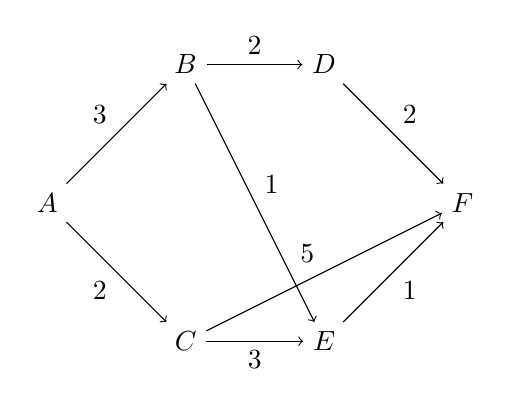
\begin{tikzpicture}[node distance=5em]
        \node (a) {$A$};
        \node (b) [right of=a, above of=a] {$B$};
        \node (c) [right of=a, below of=a] {$C$};
        \node (d) [right of=b] {$D$};
        \node (e) [right of=c] {$E$};
        \node (f) [right of=d, below of=d] {$F$};
        \draw[->] (a) to node {3} (b);
        \draw[->] (a) to node [below left]{2} (c);
        \draw[->] (b) to node {2} (d);
        \draw[->] (b) to node {1} (e);
        \draw[->] (c) to node [below]{3} (e);
        \draw[->] (c) to node {5} (f);
        \draw[->] (d) to node {2} (f);
        \draw[->] (e) to node [below right]{1} (f);
      \end{tikzpicture}
    \end{center}

  \item Multi-unit auction: $K$ units of an identical good are up for sale
    and each buyer has a valuation $v_i$ for a single item.
  \end{enumerate}
\end{exercise}

%%%%%%%%%%%%%%%
\end{spacing}
\end{document}
%%%%% FIN %%%%%
%%%%%%%%%%%%%%%